%%%%%%%%%%%%%%%%%%%%%%%%%%%%%%%%%%%%%%%%%
% Focus Beamer Presentation
% LaTeX Template
% Version 1.0 (8/8/18)
%
% This template has been downloaded from:
% http://www.LaTeXTemplates.com
%
% Original author:
% Pasquale Africa (https://github.com/elauksap/focus-beamertheme) with modifications by 
% Vel (vel@LaTeXTemplates.com)
%
% Template license:
% GNU GPL v3.0 License
%
% Important note:
% The bibliography/references need to be compiled with bibtex.
%
%%%%%%%%%%%%%%%%%%%%%%%%%%%%%%%%%%%%%%%%%

%----------------------------------------------------------------------------------------
%	PACKAGES AND OTHER DOCUMENT CONFIGURATIONS
%----------------------------------------------------------------------------------------

\documentclass{beamer}

\usetheme{focus} % Use the Focus theme supplied with the template
% Add option [numbering=none] to disable the footer progress bar
% Add option [numbering=fullbar] to show the footer progress bar as always full with a slide countx


\definecolor{main}{RGB}{55, 135, 177}
\definecolor{text}{RGB}{57, 100, 131}
\definecolor{background}{RGB}{255, 255, 255}

\addtobeamertemplate{block begin}{%
	\setlength{\textwidth}{0.9\textwidth}%
}{}

\addtobeamertemplate{block alerted begin}{%
	\setlength{\textwidth}{0.9\textwidth}%
}{}

\addtobeamertemplate{block example begin}{%
	\setlength{\textwidth}{0.9\textwidth}%
}{}

\setbeamercovered{transparent}

%------------------------------------------------

\usepackage{booktabs} % Required for better table rules
\usepackage{tikz}
\usepackage{xepersian}
\settextfont{Vazir}
\setsansfont{FreeSerif}
\renewcommand{\baselinestretch}{1.3}

\title{\rl{مسئله‌ی فروشنده‌ی دوره‌گرد}}

\subtitle{\rl{یک الگوریتمِ} PTAS \rl{برای حالت اقلیدسی}}

\author{\rl{علیرضا محمودیان}}

\titlegraphic{
\includegraphics[scale=.21]{Images/tu-logo-hckd.png}}

\institute{\rl{	دانشکده‌ی ریاضی، آمار و علومِ کامپیوتر \\ دانشگاهِ تهران}}

\date{\rl{دی ۱۳۹۷}}


\begin{document}


\begin{frame}
	\maketitle
\end{frame}

\begin{frame}{\rl{مسئله‌ی فروشنده‌ی دوره‌گرد}}
    \begin{flushright}\rl{
    	\begin{block}{مسئله}
             پیداکردنِ دورِ همیلتونی با هزینه‌ی کمینه
    	\end{block}
        $\bullet$ در حالتِ کلی تقریب‌پذیر نیست. \\
        $\bullet$ تابعِ هزینه‌ی متریک $~\leftarrow~$  تقریب با فاکتورِ ۳/۲ \\
        $\bullet$ تابعِ هزینه‌ی اقلیدسی $~\leftarrow~$ PTAS
    }\end{flushright}
\end{frame}

\begin{frame}{\rl{الگوریتمِ :PTAS ایده‌ی اصلی}}
	\begin{flushright}
		$\blacksquare$ \rl{ساختِ نمونه‌ی تقریب‌پذیر از روی نمونه‌ی اصلی} \\
		\pause
		$\bullet~~~~~~~~~$ \rl{ هزینه‌ی دورِ بهینه‌ی نمونه‌ی تقریب‌پذیر با هر تقریبِ دلخواه به\\
			$~~~~~~~~~~~$ جوابِ اصلی نزدیک می‌شود (PTAS)} \\
		\pause
		$\blacksquare$ \rl{بدست‌آوردنِ جوابِ خوش‌رفتار در زمانِ چندجمله‌ای} (DP) \\
		\pause
		$\bullet~~~~~~~~~$ \rl{جوابِ خوش‌رفتار PTAS نیست} \\
		\pause
		$\blacksquare$ \rl{وجود جوابِ PTAS با تحلیلِ تصادفی}
	\end{flushright}
\end{frame}

\section{\rl{نمونه‌ی تقریب‌پذیر}}

\begin{frame}[t]{\rl{نمونه‌ی تقریب‌پذیر}}
	\begin{flushright}\rl{
		\begin{block}{تعریف}
            \begin{enumerate}
            	\item اندازه‌ی نمونه، $n$، توانی از ۲ باشد \\
            	\pause
                \item مختصاتِ هر گره اعدادی صحیح در بازه‌ی $[0, O(n)]^d$ باشند \\
                \pause
                \item یال با هزینه‌ی کم‌تر از ۴ نداشته باشد
            \end{enumerate}
		\end{block}
	}\end{flushright}
\end{frame}

\begin{frame}[t]{\rl{نمونه‌ی تقریب‌پذیر: ساخت}}
	\rl{
		\begin{columns}[onlytextwidth]
			\column{0.4\textwidth}
			\flushleft
			% Graphic for TeX using PGF
% Title: /home/beleg/Diagram1.dia
% Creator: Dia v0.97+git
% CreationDate: Fri Dec 28 21:14:45 2018
% For: beleg
% \usepackage{tikz}
% The following commands are not supported in PSTricks at present
% We define them conditionally, so when they are implemented,
% this pgf file will use them.
\ifx\du\undefined
  \newlength{\du}
\fi
\setlength{\du}{15\unitlength}
\begin{tikzpicture}[even odd rule]
\pgftransformxscale{1.400000}
\pgftransformyscale{-1.400000}
\definecolor{dialinecolor}{rgb}{0.000000, 0.000000, 0.000000}
\pgfsetstrokecolor{dialinecolor}
\pgfsetstrokeopacity{1.000000}
\definecolor{diafillcolor}{rgb}{1.000000, 1.000000, 1.000000}
\pgfsetfillcolor{diafillcolor}
\pgfsetfillopacity{1.000000}
\pgfsetlinewidth{0.000000\du}
\pgfsetdash{}{0pt}
\pgfsetbuttcap
\pgfsetmiterjoin
\pgfsetlinewidth{0.000000\du}
\pgfsetbuttcap
\pgfsetmiterjoin
\pgfsetdash{}{0pt}
\definecolor{diafillcolor}{rgb}{0.000000, 0.000000, 0.000000}
\pgfsetfillcolor{diafillcolor}
\pgfsetfillopacity{1.000000}
\pgfpathellipse{\pgfpoint{5.326864\du}{12.267626\du}}{\pgfpoint{0.058776\du}{0\du}}{\pgfpoint{0\du}{0.058776\du}}
\pgfusepath{fill}
\definecolor{dialinecolor}{rgb}{0.000000, 0.000000, 0.000000}
\pgfsetstrokecolor{dialinecolor}
\pgfsetstrokeopacity{1.000000}
\pgfpathellipse{\pgfpoint{5.326864\du}{12.267626\du}}{\pgfpoint{0.058776\du}{0\du}}{\pgfpoint{0\du}{0.058776\du}}
\pgfusepath{stroke}
\pgfsetlinewidth{0.000000\du}
\pgfsetdash{}{0pt}
\pgfsetbuttcap
\pgfsetmiterjoin
\pgfsetlinewidth{0.000000\du}
\pgfsetbuttcap
\pgfsetmiterjoin
\pgfsetdash{}{0pt}
\definecolor{diafillcolor}{rgb}{0.000000, 0.000000, 0.000000}
\pgfsetfillcolor{diafillcolor}
\pgfsetfillopacity{1.000000}
\pgfpathellipse{\pgfpoint{5.301078\du}{7.473806\du}}{\pgfpoint{0.058776\du}{0\du}}{\pgfpoint{0\du}{0.058776\du}}
\pgfusepath{fill}
\definecolor{dialinecolor}{rgb}{0.000000, 0.000000, 0.000000}
\pgfsetstrokecolor{dialinecolor}
\pgfsetstrokeopacity{1.000000}
\pgfpathellipse{\pgfpoint{5.301078\du}{7.473806\du}}{\pgfpoint{0.058776\du}{0\du}}{\pgfpoint{0\du}{0.058776\du}}
\pgfusepath{stroke}
\pgfsetlinewidth{0.000000\du}
\pgfsetdash{}{0pt}
\pgfsetbuttcap
\pgfsetmiterjoin
\pgfsetlinewidth{0.000000\du}
\pgfsetbuttcap
\pgfsetmiterjoin
\pgfsetdash{}{0pt}
\definecolor{diafillcolor}{rgb}{0.000000, 0.000000, 0.000000}
\pgfsetfillcolor{diafillcolor}
\pgfsetfillopacity{1.000000}
\pgfpathellipse{\pgfpoint{2.501382\du}{8.272726\du}}{\pgfpoint{0.058776\du}{0\du}}{\pgfpoint{0\du}{0.058776\du}}
\pgfusepath{fill}
\definecolor{dialinecolor}{rgb}{0.000000, 0.000000, 0.000000}
\pgfsetstrokecolor{dialinecolor}
\pgfsetstrokeopacity{1.000000}
\pgfpathellipse{\pgfpoint{2.501382\du}{8.272726\du}}{\pgfpoint{0.058776\du}{0\du}}{\pgfpoint{0\du}{0.058776\du}}
\pgfusepath{stroke}
\pgfsetlinewidth{0.000000\du}
\pgfsetdash{}{0pt}
\pgfsetbuttcap
\pgfsetmiterjoin
\pgfsetlinewidth{0.000000\du}
\pgfsetbuttcap
\pgfsetmiterjoin
\pgfsetdash{}{0pt}
\definecolor{diafillcolor}{rgb}{0.000000, 0.000000, 0.000000}
\pgfsetfillcolor{diafillcolor}
\pgfsetfillopacity{1.000000}
\pgfpathellipse{\pgfpoint{3.500695\du}{10.771780\du}}{\pgfpoint{0.058776\du}{0\du}}{\pgfpoint{0\du}{0.058776\du}}
\pgfusepath{fill}
\definecolor{dialinecolor}{rgb}{0.000000, 0.000000, 0.000000}
\pgfsetstrokecolor{dialinecolor}
\pgfsetstrokeopacity{1.000000}
\pgfpathellipse{\pgfpoint{3.500695\du}{10.771780\du}}{\pgfpoint{0.058776\du}{0\du}}{\pgfpoint{0\du}{0.058776\du}}
\pgfusepath{stroke}
\pgfsetlinewidth{0.000000\du}
\pgfsetdash{}{0pt}
\pgfsetbuttcap
\pgfsetmiterjoin
\pgfsetlinewidth{0.000000\du}
\pgfsetbuttcap
\pgfsetmiterjoin
\pgfsetdash{}{0pt}
\definecolor{diafillcolor}{rgb}{0.000000, 0.000000, 0.000000}
\pgfsetfillcolor{diafillcolor}
\pgfsetfillopacity{1.000000}
\pgfpathellipse{\pgfpoint{4.620821\du}{9.464456\du}}{\pgfpoint{0.058776\du}{0\du}}{\pgfpoint{0\du}{0.058776\du}}
\pgfusepath{fill}
\definecolor{dialinecolor}{rgb}{0.000000, 0.000000, 0.000000}
\pgfsetstrokecolor{dialinecolor}
\pgfsetstrokeopacity{1.000000}
\pgfpathellipse{\pgfpoint{4.620821\du}{9.464456\du}}{\pgfpoint{0.058776\du}{0\du}}{\pgfpoint{0\du}{0.058776\du}}
\pgfusepath{stroke}
\pgfsetlinewidth{0.000000\du}
\pgfsetdash{}{0pt}
\pgfsetbuttcap
\pgfsetmiterjoin
\pgfsetlinewidth{0.000000\du}
\pgfsetbuttcap
\pgfsetmiterjoin
\pgfsetdash{}{0pt}
\definecolor{diafillcolor}{rgb}{0.000000, 0.000000, 0.000000}
\pgfsetfillcolor{diafillcolor}
\pgfsetfillopacity{1.000000}
\pgfpathellipse{\pgfpoint{7.275364\du}{8.790335\du}}{\pgfpoint{0.058776\du}{0\du}}{\pgfpoint{0\du}{0.058776\du}}
\pgfusepath{fill}
\definecolor{dialinecolor}{rgb}{0.000000, 0.000000, 0.000000}
\pgfsetstrokecolor{dialinecolor}
\pgfsetstrokeopacity{1.000000}
\pgfpathellipse{\pgfpoint{7.275364\du}{8.790335\du}}{\pgfpoint{0.058776\du}{0\du}}{\pgfpoint{0\du}{0.058776\du}}
\pgfusepath{stroke}
\pgfsetlinewidth{0.000000\du}
\pgfsetdash{}{0pt}
\pgfsetbuttcap
\pgfsetmiterjoin
\pgfsetlinewidth{0.000000\du}
\pgfsetbuttcap
\pgfsetmiterjoin
\pgfsetdash{}{0pt}
\definecolor{diafillcolor}{rgb}{0.000000, 0.000000, 0.000000}
\pgfsetfillcolor{diafillcolor}
\pgfsetfillopacity{1.000000}
\pgfpathellipse{\pgfpoint{6.357780\du}{9.697688\du}}{\pgfpoint{0.058776\du}{0\du}}{\pgfpoint{0\du}{0.058776\du}}
\pgfusepath{fill}
\definecolor{dialinecolor}{rgb}{0.000000, 0.000000, 0.000000}
\pgfsetstrokecolor{dialinecolor}
\pgfsetstrokeopacity{1.000000}
\pgfpathellipse{\pgfpoint{6.357780\du}{9.697688\du}}{\pgfpoint{0.058776\du}{0\du}}{\pgfpoint{0\du}{0.058776\du}}
\pgfusepath{stroke}
\pgfsetlinewidth{0.000000\du}
\pgfsetdash{}{0pt}
\pgfsetbuttcap
\pgfsetmiterjoin
\pgfsetlinewidth{0.000000\du}
\pgfsetbuttcap
\pgfsetmiterjoin
\pgfsetdash{}{0pt}
\definecolor{diafillcolor}{rgb}{0.000000, 0.000000, 0.000000}
\pgfsetfillcolor{diafillcolor}
\pgfsetfillopacity{1.000000}
\pgfpathellipse{\pgfpoint{7.992701\du}{10.693831\du}}{\pgfpoint{0.058776\du}{0\du}}{\pgfpoint{0\du}{0.058776\du}}
\pgfusepath{fill}
\definecolor{dialinecolor}{rgb}{0.000000, 0.000000, 0.000000}
\pgfsetstrokecolor{dialinecolor}
\pgfsetstrokeopacity{1.000000}
\pgfpathellipse{\pgfpoint{7.992701\du}{10.693831\du}}{\pgfpoint{0.058776\du}{0\du}}{\pgfpoint{0\du}{0.058776\du}}
\pgfusepath{stroke}
\pgfsetlinewidth{0.050000\du}
\pgfsetdash{}{0pt}
\pgfsetbuttcap
\pgfsetmiterjoin
\pgfsetlinewidth{0.050000\du}
\pgfsetbuttcap
\pgfsetmiterjoin
\pgfsetdash{}{0pt}
{\pgfsetcornersarced{\pgfpoint{0.000000\du}{0.000000\du}}\definecolor{dialinecolor}{rgb}{0.000000, 0.000000, 0.000000}
\pgfsetstrokecolor{dialinecolor}
\pgfsetstrokeopacity{1.000000}
\draw (2.502339\du,7.108220\du)--(2.502339\du,12.786692\du)--(7.997634\du,12.786692\du)--(7.997634\du,7.108220\du)--cycle;
}\pgfsetlinewidth{0.030000\du}
\pgfsetdash{}{0pt}
\pgfsetbuttcap
{
\definecolor{diafillcolor}{rgb}{0.000000, 0.000000, 0.000000}
\pgfsetfillcolor{diafillcolor}
\pgfsetfillopacity{1.000000}
% was here!!!
}
\definecolor{dialinecolor}{rgb}{0.000000, 0.000000, 0.000000}
\pgfsetstrokecolor{dialinecolor}
\pgfsetstrokeopacity{1.000000}
\draw (2.499297\du,6.801944\du)--(8.005526\du,6.801944\du);
\pgfsetlinewidth{0.030000\du}
\pgfsetdash{}{0pt}
\pgfsetmiterjoin
\pgfsetbuttcap
\definecolor{dialinecolor}{rgb}{0.000000, 0.000000, 0.000000}
\pgfsetstrokecolor{dialinecolor}
\pgfsetstrokeopacity{1.000000}
\draw (2.399297\du,6.701944\du)--(2.499297\du,6.801944\du)--(2.399297\du,6.901944\du);
\pgfsetlinewidth{0.030000\du}
\pgfsetdash{}{0pt}
\pgfsetmiterjoin
\pgfsetbuttcap
\definecolor{dialinecolor}{rgb}{0.000000, 0.000000, 0.000000}
\pgfsetstrokecolor{dialinecolor}
\pgfsetstrokeopacity{1.000000}
\draw (8.105526\du,6.901944\du)--(8.005526\du,6.801944\du)--(8.105526\du,6.701944\du);
\definecolor{diafillcolor}{rgb}{1.000000, 1.000000, 1.000000}
\pgfsetfillcolor{diafillcolor}
\pgfsetfillopacity{1.000000}
\fill (4.103675\du,6.521042\du)--(6.216175\du,6.521042\du)--(6.216175\du,7.036042\du)--(4.103675\du,7.036042\du)--cycle;
% setfont left to latex
\definecolor{dialinecolor}{rgb}{0.000000, 0.000000, 0.000000}
\pgfsetstrokecolor{dialinecolor}
\pgfsetstrokeopacity{1.000000}
\definecolor{diafillcolor}{rgb}{0.000000, 0.000000, 0.000000}
\pgfsetfillcolor{diafillcolor}
\pgfsetfillopacity{1.000000}
\node[anchor=base west,inner sep=0pt,outer sep=0pt,color=dialinecolor] at (4.103675\du,6.931042\du){$L = 8n/\epsilon$};
\end{tikzpicture}

			\column{0.6\textwidth}
			\flushright
			$\bullet$ به نمونه‌ی اولیه به تعدادِ کافی گره‌ی تکراری می‌افزاییم تا اندازه‌ی آن توانی از دو شود.\\
			\pause
			$\bullet$ آن را با کوچک‌ترین مربعِ ممکن محصور می‌کنیم.\\
			\pause
			$\bullet$ برای $\epsilon$ِ زوج،  نمونه را تاجایی بزرگ می‌کنیم که طولِ ضلعِ مربع برابر با
			$8n/\epsilon$ شود.\\
			\pause
			$\blacksquare$ واضح است که این کار دورِ بهینه را تغییر نمی‌دهد.
		\end{columns}
	}
\end{frame}


\begin{frame}[t]{\rl{نمونه‌ی تقریب‌پذیر: ساخت}}
	\rl{
		\begin{columns}[onlytextwidth]
			\column{0.4\textwidth}
			\flushleft
			% Graphic for TeX using PGF
% Title: /home/beleg/Documents/euc-tsp.dia
% Creator: Dia v0.97+git
% CreationDate: Sat Dec 29 02:34:16 2018
% For: beleg
% \usepackage{tikz}
% The following commands are not supported in PSTricks at present
% We define them conditionally, so when they are implemented,
% this pgf file will use them.
\ifx\du\undefined
  \newlength{\du}
\fi
\setlength{\du}{15\unitlength}
\begin{tikzpicture}[even odd rule]
\pgftransformxscale{1.400000}
\pgftransformyscale{-1.400000}
\definecolor{dialinecolor}{rgb}{0.000000, 0.000000, 0.000000}
\pgfsetstrokecolor{dialinecolor}
\pgfsetstrokeopacity{1.000000}
\definecolor{diafillcolor}{rgb}{1.000000, 1.000000, 1.000000}
\pgfsetfillcolor{diafillcolor}
\pgfsetfillopacity{1.000000}
\pgfsetlinewidth{0.000000\du}
\pgfsetdash{}{0pt}
\pgfsetbuttcap
\pgfsetmiterjoin
\pgfsetlinewidth{0.000000\du}
\pgfsetbuttcap
\pgfsetmiterjoin
\pgfsetdash{}{0pt}
\definecolor{diafillcolor}{rgb}{0.000000, 0.000000, 0.000000}
\pgfsetfillcolor{diafillcolor}
\pgfsetfillopacity{1.000000}
\pgfpathellipse{\pgfpoint{5.326866\du}{12.267576\du}}{\pgfpoint{0.058776\du}{0\du}}{\pgfpoint{0\du}{0.058776\du}}
\pgfusepath{fill}
\definecolor{dialinecolor}{rgb}{0.000000, 0.000000, 0.000000}
\pgfsetstrokecolor{dialinecolor}
\pgfsetstrokeopacity{1.000000}
\pgfpathellipse{\pgfpoint{5.326866\du}{12.267576\du}}{\pgfpoint{0.058776\du}{0\du}}{\pgfpoint{0\du}{0.058776\du}}
\pgfusepath{stroke}
\pgfsetlinewidth{0.000000\du}
\pgfsetdash{}{0pt}
\pgfsetbuttcap
\pgfsetmiterjoin
\pgfsetlinewidth{0.000000\du}
\pgfsetbuttcap
\pgfsetmiterjoin
\pgfsetdash{}{0pt}
\definecolor{diafillcolor}{rgb}{0.000000, 0.000000, 0.000000}
\pgfsetfillcolor{diafillcolor}
\pgfsetfillopacity{1.000000}
\pgfpathellipse{\pgfpoint{5.301076\du}{7.473806\du}}{\pgfpoint{0.058776\du}{0\du}}{\pgfpoint{0\du}{0.058776\du}}
\pgfusepath{fill}
\definecolor{dialinecolor}{rgb}{0.000000, 0.000000, 0.000000}
\pgfsetstrokecolor{dialinecolor}
\pgfsetstrokeopacity{1.000000}
\pgfpathellipse{\pgfpoint{5.301076\du}{7.473806\du}}{\pgfpoint{0.058776\du}{0\du}}{\pgfpoint{0\du}{0.058776\du}}
\pgfusepath{stroke}
\pgfsetlinewidth{0.000000\du}
\pgfsetdash{}{0pt}
\pgfsetbuttcap
\pgfsetmiterjoin
\pgfsetlinewidth{0.000000\du}
\pgfsetbuttcap
\pgfsetmiterjoin
\pgfsetdash{}{0pt}
\definecolor{diafillcolor}{rgb}{0.000000, 0.000000, 0.000000}
\pgfsetfillcolor{diafillcolor}
\pgfsetfillopacity{1.000000}
\pgfpathellipse{\pgfpoint{2.501386\du}{8.272726\du}}{\pgfpoint{0.058776\du}{0\du}}{\pgfpoint{0\du}{0.058776\du}}
\pgfusepath{fill}
\definecolor{dialinecolor}{rgb}{0.000000, 0.000000, 0.000000}
\pgfsetstrokecolor{dialinecolor}
\pgfsetstrokeopacity{1.000000}
\pgfpathellipse{\pgfpoint{2.501386\du}{8.272726\du}}{\pgfpoint{0.058776\du}{0\du}}{\pgfpoint{0\du}{0.058776\du}}
\pgfusepath{stroke}
\pgfsetlinewidth{0.000000\du}
\pgfsetdash{}{0pt}
\pgfsetbuttcap
\pgfsetmiterjoin
\pgfsetlinewidth{0.000000\du}
\pgfsetbuttcap
\pgfsetmiterjoin
\pgfsetdash{}{0pt}
\definecolor{diafillcolor}{rgb}{0.000000, 0.000000, 0.000000}
\pgfsetfillcolor{diafillcolor}
\pgfsetfillopacity{1.000000}
\pgfpathellipse{\pgfpoint{3.500696\du}{10.771776\du}}{\pgfpoint{0.058776\du}{0\du}}{\pgfpoint{0\du}{0.058776\du}}
\pgfusepath{fill}
\definecolor{dialinecolor}{rgb}{0.000000, 0.000000, 0.000000}
\pgfsetstrokecolor{dialinecolor}
\pgfsetstrokeopacity{1.000000}
\pgfpathellipse{\pgfpoint{3.500696\du}{10.771776\du}}{\pgfpoint{0.058776\du}{0\du}}{\pgfpoint{0\du}{0.058776\du}}
\pgfusepath{stroke}
\pgfsetlinewidth{0.000000\du}
\pgfsetdash{}{0pt}
\pgfsetbuttcap
\pgfsetmiterjoin
\pgfsetlinewidth{0.000000\du}
\pgfsetbuttcap
\pgfsetmiterjoin
\pgfsetdash{}{0pt}
\definecolor{diafillcolor}{rgb}{0.000000, 0.000000, 0.000000}
\pgfsetfillcolor{diafillcolor}
\pgfsetfillopacity{1.000000}
\pgfpathellipse{\pgfpoint{4.620816\du}{9.464456\du}}{\pgfpoint{0.058776\du}{0\du}}{\pgfpoint{0\du}{0.058776\du}}
\pgfusepath{fill}
\definecolor{dialinecolor}{rgb}{0.000000, 0.000000, 0.000000}
\pgfsetstrokecolor{dialinecolor}
\pgfsetstrokeopacity{1.000000}
\pgfpathellipse{\pgfpoint{4.620816\du}{9.464456\du}}{\pgfpoint{0.058776\du}{0\du}}{\pgfpoint{0\du}{0.058776\du}}
\pgfusepath{stroke}
\pgfsetlinewidth{0.000000\du}
\pgfsetdash{}{0pt}
\pgfsetbuttcap
\pgfsetmiterjoin
\pgfsetlinewidth{0.000000\du}
\pgfsetbuttcap
\pgfsetmiterjoin
\pgfsetdash{}{0pt}
\definecolor{diafillcolor}{rgb}{0.000000, 0.000000, 0.000000}
\pgfsetfillcolor{diafillcolor}
\pgfsetfillopacity{1.000000}
\pgfpathellipse{\pgfpoint{7.275366\du}{8.790336\du}}{\pgfpoint{0.058776\du}{0\du}}{\pgfpoint{0\du}{0.058776\du}}
\pgfusepath{fill}
\definecolor{dialinecolor}{rgb}{0.000000, 0.000000, 0.000000}
\pgfsetstrokecolor{dialinecolor}
\pgfsetstrokeopacity{1.000000}
\pgfpathellipse{\pgfpoint{7.275366\du}{8.790336\du}}{\pgfpoint{0.058776\du}{0\du}}{\pgfpoint{0\du}{0.058776\du}}
\pgfusepath{stroke}
\pgfsetlinewidth{0.000000\du}
\pgfsetdash{}{0pt}
\pgfsetbuttcap
\pgfsetmiterjoin
\pgfsetlinewidth{0.000000\du}
\pgfsetbuttcap
\pgfsetmiterjoin
\pgfsetdash{}{0pt}
\definecolor{diafillcolor}{rgb}{0.000000, 0.000000, 0.000000}
\pgfsetfillcolor{diafillcolor}
\pgfsetfillopacity{1.000000}
\pgfpathellipse{\pgfpoint{6.357776\du}{9.697686\du}}{\pgfpoint{0.058776\du}{0\du}}{\pgfpoint{0\du}{0.058776\du}}
\pgfusepath{fill}
\definecolor{dialinecolor}{rgb}{0.000000, 0.000000, 0.000000}
\pgfsetstrokecolor{dialinecolor}
\pgfsetstrokeopacity{1.000000}
\pgfpathellipse{\pgfpoint{6.357776\du}{9.697686\du}}{\pgfpoint{0.058776\du}{0\du}}{\pgfpoint{0\du}{0.058776\du}}
\pgfusepath{stroke}
\pgfsetlinewidth{0.000000\du}
\pgfsetdash{}{0pt}
\pgfsetbuttcap
\pgfsetmiterjoin
\pgfsetlinewidth{0.000000\du}
\pgfsetbuttcap
\pgfsetmiterjoin
\pgfsetdash{}{0pt}
\definecolor{diafillcolor}{rgb}{0.000000, 0.000000, 0.000000}
\pgfsetfillcolor{diafillcolor}
\pgfsetfillopacity{1.000000}
\pgfpathellipse{\pgfpoint{7.992696\du}{10.693876\du}}{\pgfpoint{0.058776\du}{0\du}}{\pgfpoint{0\du}{0.058776\du}}
\pgfusepath{fill}
\definecolor{dialinecolor}{rgb}{0.000000, 0.000000, 0.000000}
\pgfsetstrokecolor{dialinecolor}
\pgfsetstrokeopacity{1.000000}
\pgfpathellipse{\pgfpoint{7.992696\du}{10.693876\du}}{\pgfpoint{0.058776\du}{0\du}}{\pgfpoint{0\du}{0.058776\du}}
\pgfusepath{stroke}
\pgfsetlinewidth{0.050000\du}
\pgfsetdash{}{0pt}
\pgfsetbuttcap
\pgfsetmiterjoin
\pgfsetlinewidth{0.050000\du}
\pgfsetbuttcap
\pgfsetmiterjoin
\pgfsetdash{}{0pt}
{\pgfsetcornersarced{\pgfpoint{0.000000\du}{0.000000\du}}\definecolor{dialinecolor}{rgb}{0.000000, 0.000000, 0.000000}
\pgfsetstrokecolor{dialinecolor}
\pgfsetstrokeopacity{1.000000}
\draw (2.502340\du,7.108220\du)--(2.502340\du,12.786692\du)--(7.997635\du,12.786692\du)--(7.997635\du,7.108220\du)--cycle;
}\pgfsetlinewidth{0.040000\du}
\pgfsetdash{}{0pt}
\pgfsetbuttcap
{
\definecolor{diafillcolor}{rgb}{0.000000, 0.000000, 0.000000}
\pgfsetfillcolor{diafillcolor}
\pgfsetfillopacity{1.000000}
% was here!!!
\definecolor{dialinecolor}{rgb}{0.000000, 0.000000, 0.000000}
\pgfsetstrokecolor{dialinecolor}
\pgfsetstrokeopacity{1.000000}
\draw (5.249990\du,12.786700\du)--(5.249990\du,7.108220\du);
}
\pgfsetlinewidth{0.040000\du}
\pgfsetdash{}{0pt}
\pgfsetbuttcap
{
\definecolor{diafillcolor}{rgb}{0.000000, 0.000000, 0.000000}
\pgfsetfillcolor{diafillcolor}
\pgfsetfillopacity{1.000000}
% was here!!!
\definecolor{dialinecolor}{rgb}{0.000000, 0.000000, 0.000000}
\pgfsetstrokecolor{dialinecolor}
\pgfsetstrokeopacity{1.000000}
\draw (3.939970\du,12.798000\du)--(3.939970\du,7.119530\du);
}
\pgfsetlinewidth{0.040000\du}
\pgfsetdash{}{0pt}
\pgfsetbuttcap
{
\definecolor{diafillcolor}{rgb}{0.000000, 0.000000, 0.000000}
\pgfsetfillcolor{diafillcolor}
\pgfsetfillopacity{1.000000}
% was here!!!
\definecolor{dialinecolor}{rgb}{0.000000, 0.000000, 0.000000}
\pgfsetstrokecolor{dialinecolor}
\pgfsetstrokeopacity{1.000000}
\draw (6.611970\du,12.818800\du)--(6.611970\du,7.140330\du);
}
\pgfsetlinewidth{0.040000\du}
\pgfsetdash{}{0pt}
\pgfsetbuttcap
{
\definecolor{diafillcolor}{rgb}{0.000000, 0.000000, 0.000000}
\pgfsetfillcolor{diafillcolor}
\pgfsetfillopacity{1.000000}
% was here!!!
\definecolor{dialinecolor}{rgb}{0.000000, 0.000000, 0.000000}
\pgfsetstrokecolor{dialinecolor}
\pgfsetstrokeopacity{1.000000}
\draw (2.499970\du,8.527530\du)--(7.995260\du,8.527530\du);
}
\pgfsetlinewidth{0.040000\du}
\pgfsetdash{}{0pt}
\pgfsetmiterjoin
\pgfsetbuttcap
\definecolor{dialinecolor}{rgb}{0.000000, 0.000000, 0.000000}
\pgfsetstrokecolor{dialinecolor}
\pgfsetstrokeopacity{1.000000}
\pgfpathmoveto{\pgfpoint{2.502340\du}{9.947460\du}}
\pgfpathlineto{\pgfpoint{7.997630\du}{9.947460\du}}
\pgfpathlineto{\pgfpoint{2.502340\du}{9.947460\du}}
\pgfpathmoveto{\pgfpoint{2.499970\du}{11.332300\du}}
\pgfpathlineto{\pgfpoint{7.995260\du}{11.332300\du}}
\pgfpathlineto{\pgfpoint{2.499970\du}{11.332300\du}}
\pgfusepath{stroke}
\pgfsetlinewidth{0.000000\du}
\pgfsetdash{{\pgflinewidth}{0.200000\du}}{0cm}
\pgfsetbuttcap
{
\definecolor{diafillcolor}{rgb}{0.000000, 0.000000, 0.000000}
\pgfsetfillcolor{diafillcolor}
\pgfsetfillopacity{1.000000}
% was here!!!
\definecolor{dialinecolor}{rgb}{0.000000, 0.000000, 0.000000}
\pgfsetstrokecolor{dialinecolor}
\pgfsetstrokeopacity{1.000000}
\draw (5.249988\du,9.947456\du)--(5.249988\du,9.947456\du);
}
\pgfsetlinewidth{0.050000\du}
\pgfsetdash{{\pgflinewidth}{0.100000\du}}{0cm}
\pgfsetbuttcap
{
\definecolor{diafillcolor}{rgb}{1.000000, 0.000000, 0.000000}
\pgfsetfillcolor{diafillcolor}
\pgfsetfillopacity{1.000000}
% was here!!!
\pgfsetarrowsend{stealth}
\definecolor{dialinecolor}{rgb}{1.000000, 0.000000, 0.000000}
\pgfsetstrokecolor{dialinecolor}
\pgfsetstrokeopacity{1.000000}
\draw (6.317392\du,9.655120\du)--(5.247615\du,8.527530\du);
}
\pgfsetlinewidth{0.050000\du}
\pgfsetdash{{\pgflinewidth}{0.100000\du}}{0cm}
\pgfsetbuttcap
{
\definecolor{diafillcolor}{rgb}{1.000000, 0.000000, 0.000000}
\pgfsetfillcolor{diafillcolor}
\pgfsetfillopacity{1.000000}
% was here!!!
\pgfsetarrowsend{stealth}
\definecolor{dialinecolor}{rgb}{1.000000, 0.000000, 0.000000}
\pgfsetstrokecolor{dialinecolor}
\pgfsetstrokeopacity{1.000000}
\draw (4.587380\du,9.418582\du)--(3.936042\du,8.524952\du);
}
\pgfsetlinewidth{0.050000\du}
\pgfsetdash{{\pgflinewidth}{0.100000\du}}{0cm}
\pgfsetbuttcap
{
\definecolor{diafillcolor}{rgb}{1.000000, 0.000000, 0.000000}
\pgfsetfillcolor{diafillcolor}
\pgfsetfillopacity{1.000000}
% was here!!!
\pgfsetarrowsend{stealth}
\definecolor{dialinecolor}{rgb}{1.000000, 0.000000, 0.000000}
\pgfsetstrokecolor{dialinecolor}
\pgfsetstrokeopacity{1.000000}
\draw (7.334143\du,8.790336\du)--(6.649235\du,8.508509\du);
}
\pgfsetlinewidth{0.050000\du}
\pgfsetdash{{\pgflinewidth}{0.100000\du}}{0cm}
\pgfsetbuttcap
{
\definecolor{diafillcolor}{rgb}{1.000000, 0.000000, 0.000000}
\pgfsetfillcolor{diafillcolor}
\pgfsetfillopacity{1.000000}
% was here!!!
\pgfsetarrowsend{stealth}
\definecolor{dialinecolor}{rgb}{1.000000, 0.000000, 0.000000}
\pgfsetstrokecolor{dialinecolor}
\pgfsetstrokeopacity{1.000000}
\draw (7.940784\du,10.667020\du)--(6.611970\du,9.979565\du);
}
\pgfsetlinewidth{0.050000\du}
\pgfsetdash{{\pgflinewidth}{0.100000\du}}{0cm}
\pgfsetbuttcap
{
\definecolor{diafillcolor}{rgb}{1.000000, 0.000000, 0.000000}
\pgfsetfillcolor{diafillcolor}
\pgfsetfillopacity{1.000000}
% was here!!!
\pgfsetarrowsend{stealth}
\definecolor{dialinecolor}{rgb}{1.000000, 0.000000, 0.000000}
\pgfsetstrokecolor{dialinecolor}
\pgfsetstrokeopacity{1.000000}
\draw (5.323071\du,12.209705\du)--(5.267973\du,11.369694\du);
}
\pgfsetlinewidth{0.050000\du}
\pgfsetdash{{\pgflinewidth}{0.100000\du}}{0cm}
\pgfsetbuttcap
{
\definecolor{diafillcolor}{rgb}{1.000000, 0.000000, 0.000000}
\pgfsetfillcolor{diafillcolor}
\pgfsetfillopacity{1.000000}
% was here!!!
\pgfsetarrowsend{stealth}
\definecolor{dialinecolor}{rgb}{1.000000, 0.000000, 0.000000}
\pgfsetstrokecolor{dialinecolor}
\pgfsetstrokeopacity{1.000000}
\draw (3.455361\du,10.734344\du)--(2.502340\du,9.947456\du);
}
\pgfsetlinewidth{0.050000\du}
\pgfsetdash{{\pgflinewidth}{0.100000\du}}{0cm}
\pgfsetbuttcap
{
\definecolor{diafillcolor}{rgb}{1.000000, 0.000000, 0.000000}
\pgfsetfillcolor{diafillcolor}
\pgfsetfillopacity{1.000000}
% was here!!!
\pgfsetarrowsend{stealth}
\definecolor{dialinecolor}{rgb}{1.000000, 0.000000, 0.000000}
\pgfsetstrokecolor{dialinecolor}
\pgfsetstrokeopacity{1.000000}
\draw (2.501386\du,8.213950\du)--(2.502340\du,7.108220\du);
}
\pgfsetlinewidth{0.050000\du}
\pgfsetdash{{\pgflinewidth}{0.100000\du}}{0cm}
\pgfsetbuttcap
{
\definecolor{diafillcolor}{rgb}{1.000000, 0.000000, 0.000000}
\pgfsetfillcolor{diafillcolor}
\pgfsetfillopacity{1.000000}
% was here!!!
\pgfsetarrowsend{stealth}
\definecolor{dialinecolor}{rgb}{1.000000, 0.000000, 0.000000}
\pgfsetstrokecolor{dialinecolor}
\pgfsetstrokeopacity{1.000000}
\draw (5.292994\du,7.415969\du)--(5.249988\du,7.108220\du);
}
\pgfsetlinewidth{0.030000\du}
\pgfsetdash{}{0pt}
\pgfsetbuttcap
{
\definecolor{diafillcolor}{rgb}{0.000000, 0.000000, 0.000000}
\pgfsetfillcolor{diafillcolor}
\pgfsetfillopacity{1.000000}
% was here!!!
}
\definecolor{dialinecolor}{rgb}{0.000000, 0.000000, 0.000000}
\pgfsetstrokecolor{dialinecolor}
\pgfsetstrokeopacity{1.000000}
\draw (8.376944\du,8.526556\du)--(8.386629\du,9.959947\du);
\pgfsetlinewidth{0.030000\du}
\pgfsetdash{}{0pt}
\pgfsetmiterjoin
\pgfsetbuttcap
\definecolor{dialinecolor}{rgb}{0.000000, 0.000000, 0.000000}
\pgfsetstrokecolor{dialinecolor}
\pgfsetstrokeopacity{1.000000}
\draw (8.476266\du,8.425882\du)--(8.376944\du,8.526556\du)--(8.276270\du,8.427233\du);
\pgfsetlinewidth{0.030000\du}
\pgfsetdash{}{0pt}
\pgfsetmiterjoin
\pgfsetbuttcap
\definecolor{dialinecolor}{rgb}{0.000000, 0.000000, 0.000000}
\pgfsetstrokecolor{dialinecolor}
\pgfsetstrokeopacity{1.000000}
\draw (8.287307\du,10.060620\du)--(8.386629\du,9.959947\du)--(8.487302\du,10.059269\du);
\definecolor{diafillcolor}{rgb}{1.000000, 1.000000, 1.000000}
\pgfsetfillcolor{diafillcolor}
\pgfsetfillopacity{1.000000}
\fill (8.127838\du,9.034179\du)--(8.652838\du,9.034179\du)--(8.652838\du,9.514179\du)--(8.127838\du,9.514179\du)--cycle;
% setfont left to latex
\definecolor{dialinecolor}{rgb}{0.000000, 0.000000, 0.000000}
\pgfsetstrokecolor{dialinecolor}
\pgfsetstrokeopacity{1.000000}
\definecolor{diafillcolor}{rgb}{0.000000, 0.000000, 0.000000}
\pgfsetfillcolor{diafillcolor}
\pgfsetfillopacity{1.000000}
\node[anchor=base west,inner sep=0pt,outer sep=0pt,color=dialinecolor] at (8.127838\du,9.416679\du){$~4$};
\end{tikzpicture}

			\column{0.6\textwidth}
			\flushright
			$\bullet$ هر گره را به مختصاتِ مضربِ ۴ قبلی می‌بریم.\\
			\pause
			$\blacksquare$ هر گره حداکثر ۴ واحد جابه‌جا می‌شود.\\
			\pause
			$\blacksquare$ هزینه‌ی هر یال حداکثر ۸ واحد تغییر می‌کند.\\
			\pause
			$\blacksquare$ هزینه‌ی یک دورِ همیلتونی حداکثر $8 n = \epsilon L$ تغییر می‌کند.
		\end{columns}
	}
\end{frame}

\begin{frame}[t]{\rl{نمونه‌ی تقریب‌پذیر: تقریبِ دل‌حواه}}
	\rl{
		\begin{block}{تمرین ۱}
			برای هر نمونه‌ی دل‌خواهِ ETSP، جوابِ نمونه‌ی تقریب‌پذیر، $(1+\epsilon)$-تقریبِ جوابِ اصلی برای هر $\epsilon$ِ دل‌خواه است.
		\end{block}
	\begin{flushright}
		\pause
		\emph{برهان:}
		\[ L \leq OPT_{Orig} \]
		\[ OPT_{Apx} - OPT_{Orig} \leq \epsilon L \]
		\[ \Rightarrow OPT_{Apx} \leq (1 + \epsilon) OPT_{Orig}  ~~~\square \]
		\\
		\pause
		$\bullet$ پس از این بدون کاستن از کلیت، فرض می‌کنیم نمونه تقریب‌پذیر است.
	\end{flushright}
	}
\end{frame}

\section{\rl{جوابِ خوش‌رفتار}}

\begin{frame}[t]{\rl{ تقسیم‌بندیِ پایه}}
	\begin{columns}[onlytextwidth]
		\column{0.5\textwidth}
		\flushleft
		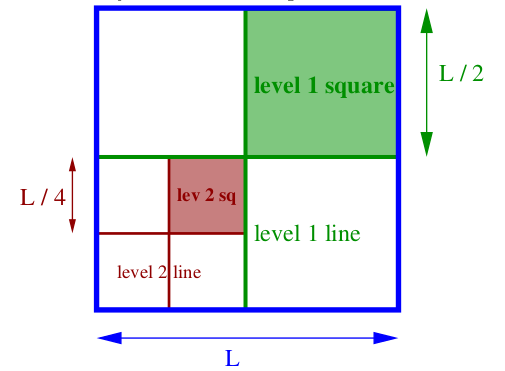
\includegraphics[width=\linewidth]{Images/levels.png}
		\column{0.5\textwidth}
		\flushright
		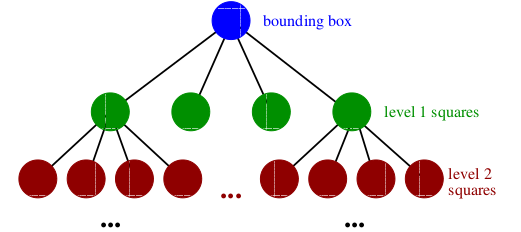
\includegraphics[width=\linewidth]{Images/tree.png}
	\end{columns}
	\rl{
	\begin{flushright}
		$\bullet$ مربعِ نمونه را به صورتِ بازگشتی به چهار مربعِ اصلی تقسیم می‌کنیم.\\
		\pause
		$\bullet$ چون $L$ توانی از ۲ است، پس از $lg(L) = O(lg(n))$ سطح به مربع‌های اصلیِ یکه می‌رسیم.\\
		\pause
		$\bullet$ به این ساختار، تقسیم‌بندیِ پایه می‌گوییم.
	\end{flushright}
	}
\end{frame}

\begin{frame}[t]{\rl{ درگاه‌ها}}
	\begin{columns}[onlytextwidth]
		\column{0.5\textwidth}
		\flushleft
		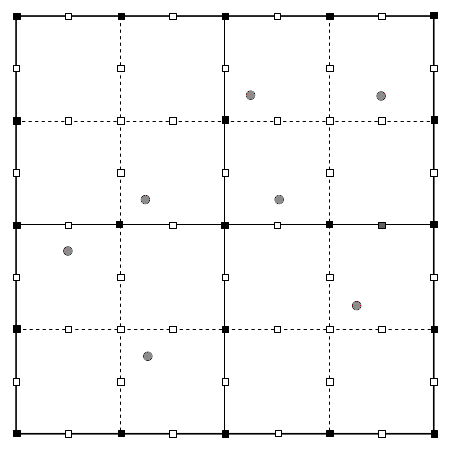
\includegraphics[width=\linewidth]{Images/portals.png}
		\column{0.5\textwidth}
		\flushright
		\rl{
		\begin{flushright}
			$\bullet$ توانی از ۲ از بازه‌ی $[lg(L)/\epsilon, 2lg(L)/\epsilon]$ انتخاب کرده و آن را $m$ می‌نامیم.\\
			\pause
			$\bullet$ روی خطوطِ سطحِ $i$-ام، $2m^i$ درگاه با فاصله‌ی برابر اضافه می‌کنیم.\\
			\pause
			$\bullet$ هر مربعِ اصلیِ سطحِ $i$-ام ۴ درگاه در گوشه‌ها و $m-1$ درگاه روی هر ضلع خواهد داشت.\\
			\pause
			$\bullet$ مربعِ بزرگ‌تر آن‌ها را بامربع‌های درونش به اشتراک می‌گذارد.
		\end{flushright}
		}
	\end{columns}
\end{frame}

\begin{frame}[t]{\rl{دورِ خوش‌رفتار}}
	\begin{flushright} \rl{
		\begin{block}{تعریف}
			\begin{enumerate}
				\item دقیقاً یک بار از هر گره‌ی اصلی عبور کند. \\
				\pause
				\item حداکثر دو بار از هر درگاه عبور کند. \\
				\pause
				\item تنها در درگاه‌ها خطوطِ تقسیم را قطع کند. \\
				\pause
				\item تنها در درگاه‌ها خودش را قطع کند.
			\end{enumerate}
		\end{block}
		\pause
		\emph{لم ۲}$\bullet$ به دلیلِ خاصیتِ مثلثی، ویژگیِ ۲ را می‌توان به کمکِ میانبرزدن تضمین کرد.
	}\end{flushright}
\end{frame}


\begin{frame}[t]{\rl{دورِ خوش‌رفتار}}
	\begin{columns}[onlytextwidth]
		\column{0.6\textwidth}
		\flushleft
		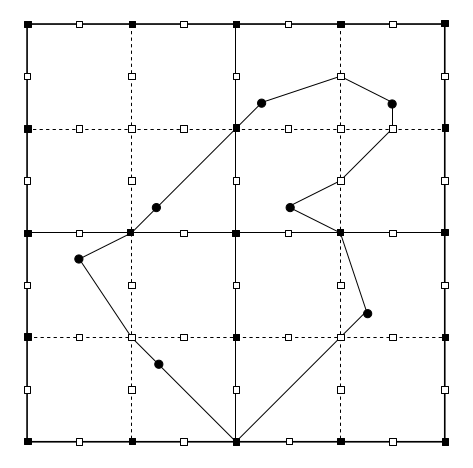
\includegraphics[width=\linewidth]{Images/route.png}
		\column{0.4\textwidth}
		\flushright \rl{
			مثال ( $m = 2$ )
		}
	\end{columns}
\end{frame}

\begin{frame}[t]{\rl{دورِ خوش‌رفتار}}
	\begin{flushright}
			\begin{exampleblock}{\rl{لم ۳}}
		\rl{		دورِ خوش‌رفتارِ بهینه در زمانِ چندجمله‌ای نسبت به اندازه‌ی ورودی قابلِ محاسبه است.}
			\end{exampleblock}
			\pause
			\emph{\rl{برهان:}}\\
			\rl{فرض کنید $\tau$ چنین دوری باشد. \\
				اولاً دقت کنید تعدادِ مربع‌های اصلی $O(n)$ است.  ابتدا حالاتِ مختلفِ قطعاتِ $\tau$ که می‌تواند داخلِ یک مربعِ اصلی باشد را می‌شماریم.}
	\end{flushright}
\end{frame}

\begin{frame}[t]{\rl{دورِ خوش‌رفتار: اثباتِ لمِ ۳}}
	\flushright{\rl { $\bullet$
			درگاه‌های ورودی/خروجی
			 $\times$ 
			   جفت‌های ممکن
			  $=$ 
			 حالاتِ مختلفِ
		  }}
	\begin{columns}[onlytextwidth]
		\column{0.4\textwidth}
		\flushleft
		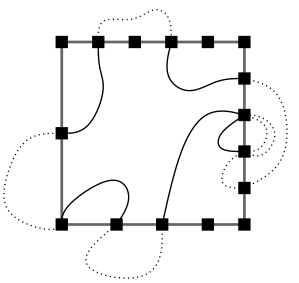
\includegraphics[width=\linewidth]{Images/pairs.png}
		\column{0.6\textwidth}
		\flushright \rl{
			$\bullet$ هر مربعِ اصلی حداکثر $4m$ درگاه دارد.\\
			\pause
			$\bullet$ هر درگاه ۰، ۱ یا ۲ بار استفاده می‌شود.\\
			\pause
			$\Leftarrow$ تعداد حالاتِ مختلفِ استفاده درگاه‌ها برای ورود/خروجِ $ \geq \tau$
			\[ 3^{4m} = n^{O(1/\epsilon	)} \]
		}
	\end{columns}
\end{frame}

\begin{frame}[t]{\rl{دورِ خوش‌رفتار: اثباتِ لمِ ۳}}
	\flushright{\rl { $\bullet$
			درگاه‌های ورودی/خروجی
			$\times$ 
			جفت‌های ممکن
			$=$ 
			حالاتِ مختلفِ
	}}
	\begin{columns}[onlytextwidth]
		\column{0.4\textwidth}
		\flushleft
		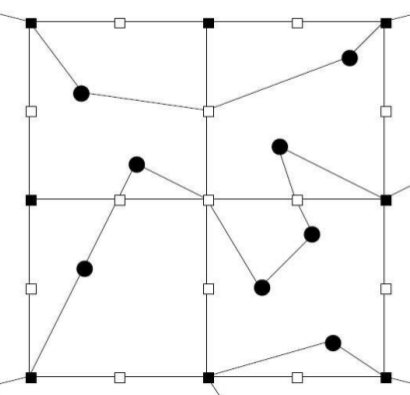
\includegraphics[width=\linewidth]{Images/paths.png}
		\column{0.6\textwidth}
		\flushright \rl{
			$\bullet$ مسیر اصلی نمی‌تواند خود را قطع کند.\\
			\pause
			$\bullet$ ورود و خروجِ $\tau$ از طریقِ درگاه‌ها تابعِ قاعده‌ی دایک خواهد بود.\\
			\pause
			$\Leftarrow$ تعداد حالاتِ مختلفِ جفت‌شدنِ درگاه‌ها $\geq$
			\[ C_{4m} = 2^{O(m)} = n^{O(1/\epsilon	)} \]
		}
	\end{columns}
\end{frame}

\begin{frame}[t]{\rl{دورِ خوش‌رفتار: یافتن بهینه}}
	\begin{flushright}\rl{
		\begin{block}{الگوریتمِ \lr{dynamic programming}}
			\begin{enumerate}
				\item  برای هر مربعِ اصلی در درختِ تقسیم‌بندیِ پایه \\
				\pause
				\item مختصاتِ هر گره اعدادی صحیح در بازه‌ی $[0, O(n)]^d$ باشند \\
				\pause
				\item یال با هزینه‌ی کم‌تر از ۴ نداشته باشد
			\end{enumerate}
		\end{block}
}\end{flushright}
\end{frame}

\begin{frame}[noframenumbering]{\rl{نوآوری‌های اخیر}}
	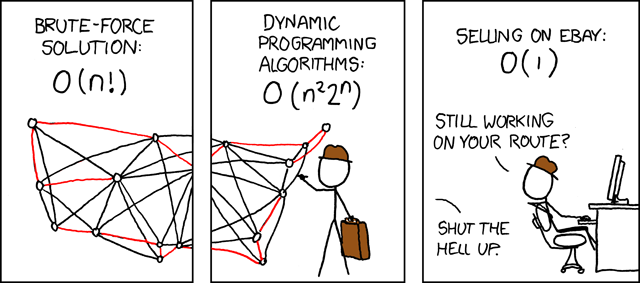
\includegraphics[width=\linewidth]{Images/travelling_salesman_problem.png}
\end{frame}

\end{document}
